% !TeX root = ../main.tex

\chapter{相关工作}

\section{基于OCC方法的设计(Tapir)}
Tapir 是第一个考虑将并发控制和共识协议进行合并设计的工作。为了迎合现代存储系统可拓展性和高可用性的特点,一般地,设计者将数据划分为多个shard储存,并且每个shard存有多个备份。在Tapir被提出之前,人们通常采用分层式的结构,为例支持事务之间的隔离性,必须实现一个分布式的事务并发控制机制,同时为了确保跨shard的原子性和副本之间一致性,必须实现一个副本间的共识协议,来确保至少大多数副本(majority)能够正确的收到事务,并按照相同或等价的序列执行。正如下图所示,这些系统通常将用于原子性保证和并发控制的事务协议(2PC+CC)置于分布式共识协议。

\begin{figure}[htb]
  \centering
  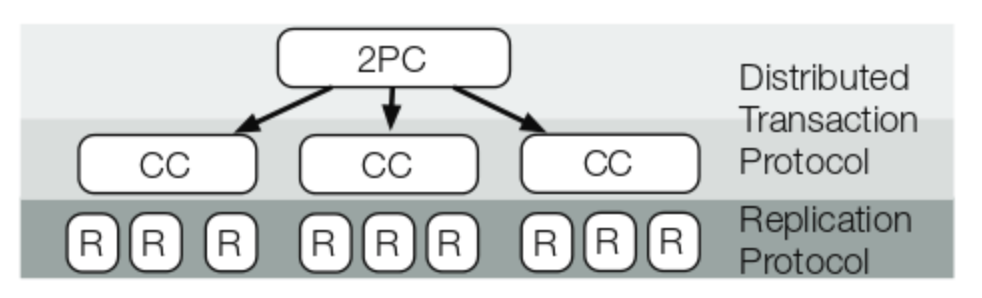
\includegraphics[width=0.6\textwidth]{Layer.png}
  \caption{分层设计模型}
  \label{fig:badge}
\end{figure}

\begin{figure}[htb]
  \centering
  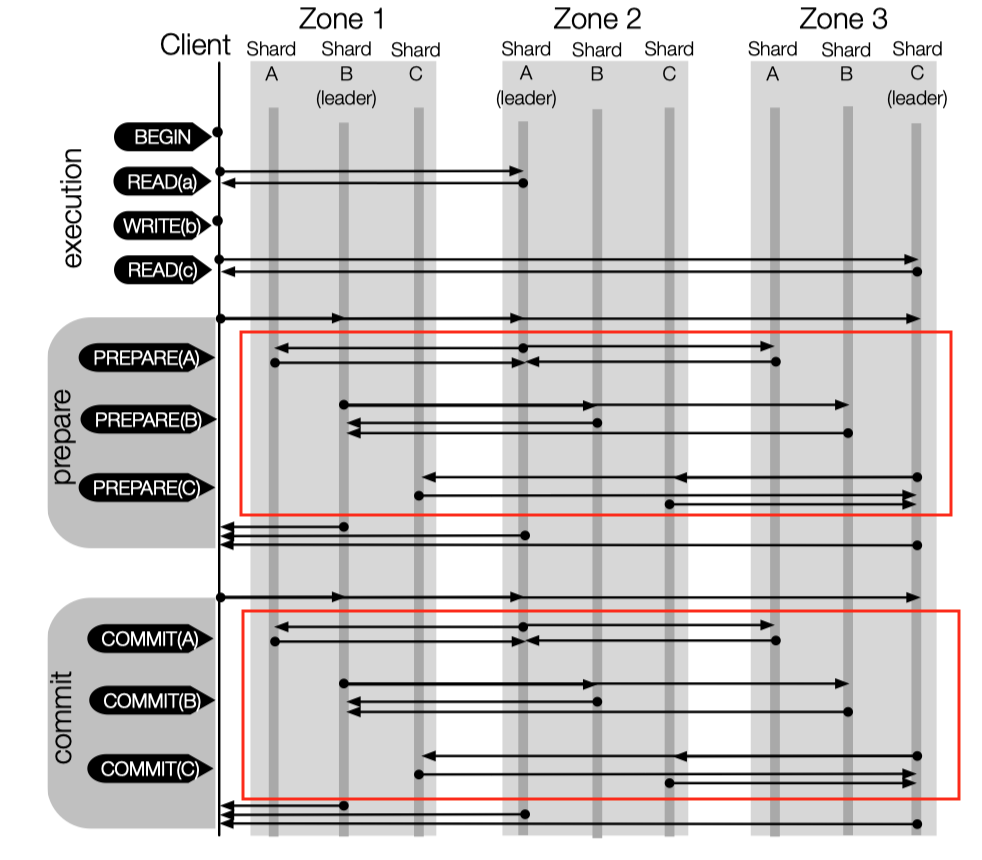
\includegraphics[width=0.77\textwidth]{Spanner.png}
  \caption{Google Spanner采用的架构}
  \label{fig:badge}
\end{figure}

Tapir系统设计设计的初衷是他观察到层次化的设计结构带来了冗余。共识协议使得同一个shard内的所有副本的事务序列化,而事务协议使得跨shard之间的事务序列化,这使得共识协议层的一些协同是冗余的,不必要的。作者以Google Spanner为例,Google Spanner的流程图如上所示。他认为图中红色方框标注的信息交换是冗余的(对应同一shard的多个副本之间的交互)。

Tapir通过采用非一致的共识协议和乐观控制协议(OCC)来消除这种冗余,虽然使用了非一致性的副本设计,但Tapir在应用层仍然能够提供强一致性的服务(线性化所有读-写事务,并支持全局的一致性读取事务)。Tapir利用了非一致性的副本来提供正常情况下可以在一个RTT(Round-Trip)下完成的读-写事务。(对比分层式设计,则至少需要两个RTT。)

具体来说,Tapir的非一致性副本协议,依赖于用户或应用层的设计来调和不一致的副本带来的问题。提供了两种操作指令。

\begin{itemize}
\item consensus
\item inconsistent
\end{itemize}

consensus和inconsistent指令下,副本都可以按照任意顺序执行事务。但是consensus指令会要求副本最终返回一个唯一的结果,即保证所有副本处于最终状态。在应用层代码中开发者可以使用consensus指令来要求系统达到一个同步的状态(类似于同步障)。

非一致性副本\cite{Consistencymodel}的设计取缔了同步的磁盘读写,假设每个shard有2f+1个副本,协议保证了只有收到大多数副本的回复的结果时(f+1)才会回复给应用层(虽然这些结果可能是冲突的),这样确保了容错机制的实现,即保证了大多数机器在同步后都能得到正确结果。

\begin{figure}[htb]
  \centering
  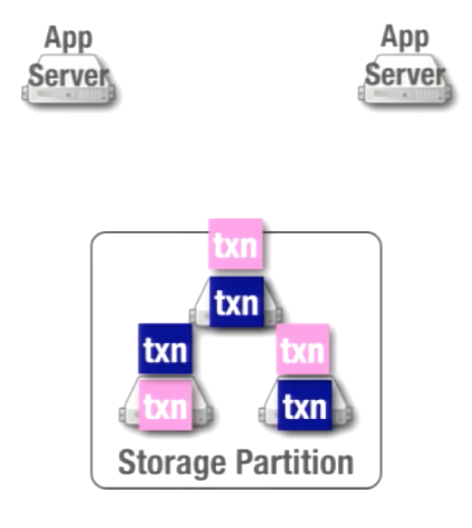
\includegraphics[width=0.35\textwidth]{Tapir.png}
  \caption{Tapir的原子性冲突检测方法}
  \label{fig:badge}
\end{figure}

那么Tapir是如何处理事务之间的冲突的呢(对于违反原子性的情况)?首先,冲突发生在多个事务同时访问某个数据的时候(并且不都是读取任务),由于Tapir保证了至少f+1个副本收到了每个事务请求,两个相互冲突的事务就必然会落到同一台机器上。如上图所示,蓝色和粉色以及橙色是冲突的三个事务,他们都被分配到了三个副本的其中两个上。这保证了Tapir能够完成冲突检测,因为遵从乐观并发控制协议,在同时收到冲突事务的副本上,他们都会被放弃提交,这样一来,相互冲突的事务中的任何一个都没发在大多数副本(f+1)上完成,从而应用层会认为事务没有执行成功

如何确保冲突的事务被序列化呢(对于并发控制)?Tapir采用了宽松的时间戳办法,对于全局事务,应用层在产生事务时会附带一个近似的时间戳,时间戳的顺序决定了序列化的顺序。那对于同一时间戳的事务又如何处理呢?由于很难实现完全同步的时钟,同一shard的不同副本可能以不同的顺序执行了两个事务,此时不同的副本可能返回给应用层协议不同的结果。此时,需要用户层协议选择其中一个结果作为最终结果,并将此结果告知有冲突结果的副本,以此来保证序列化的实现。注意,同原子性保证一样,f+1保证了一定存在一个序列化的结果。如下图:

\begin{figure}[htb]
  \centering
  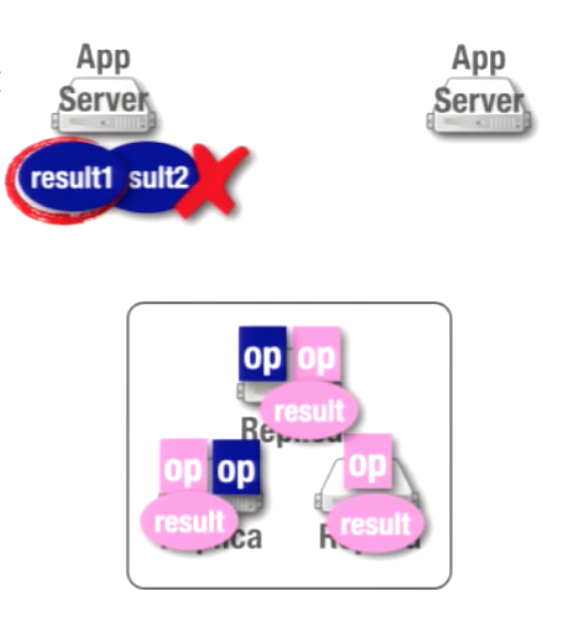
\includegraphics[width=0.35\textwidth]{IR.png}
  \caption{Tapir的序列化方法}
  \label{fig:badge}
\end{figure}

如何保证副本之间的最终一致性?Tapir采用了Multi-version的设计,并且为每个version附带时间戳,因此,可以通过副本之间的定时交互,来得到确实的version。例如:在某次提交中,某个副本不在f+1的范围中,那么他可能会丢失那个事务的提交信息。而通过与其他副本的交互,可以保证最终一致性。

如何确保用户不会读到陈旧数据?非一致性的副本设计,使得一个副本很可能不能完全看到所有的事物信息,在达到最终一致性之前,用户访问副本就会读取到陈旧的数据。但同时由于用户要在至少f+1个副本上提交事务,OCC就会检测发现这个事务之前有过数据更新,该事务读取到的数据是陈旧数据,因此会被放弃提交。显然,这种设计会给系统带来很高的放弃率。

由此,我们可以得出一个结论,就是Tapir使用于冲突较少的情景并且依赖于应用层的额外设计,因为冲突很多就会导致很高的放弃率(Abort Rate),这是由于OCC本身的性质所导致的,而这会导致系统性能变差。

\section{基于到达序的设计(Janus)}

Janus的核心出发点和Tapir一样,采用一体化的设计模型,来减少不必要的跨地区协作。与Tapir不同,Janus不需要时间戳来决定执行顺序,他使用每个副本收到事务的顺序来决定事务的执行顺序。基于到达序的序列化方法,会使得用户先发出的事务可能被后执行,因此其不能保证因果一致性。

Janus的副本会使用一张依赖图来追踪冲突事务的依赖关系,每个参与某一事务的副本都会在本地计算该事务的依赖关系,并在开始执行该事务前将其加入到依赖图中。这一步,实际完成了每个副本对事务的序列化。但是由于每个副本根据自己的到达序添加依赖项,每一个副本产生的依赖图不一定相同。因此,需要事务的组织者判断,并选择一种依赖顺序。

具体来说,janus将协议分为三个阶段,如下图所示。

\begin{figure}[htb]
  \centering
  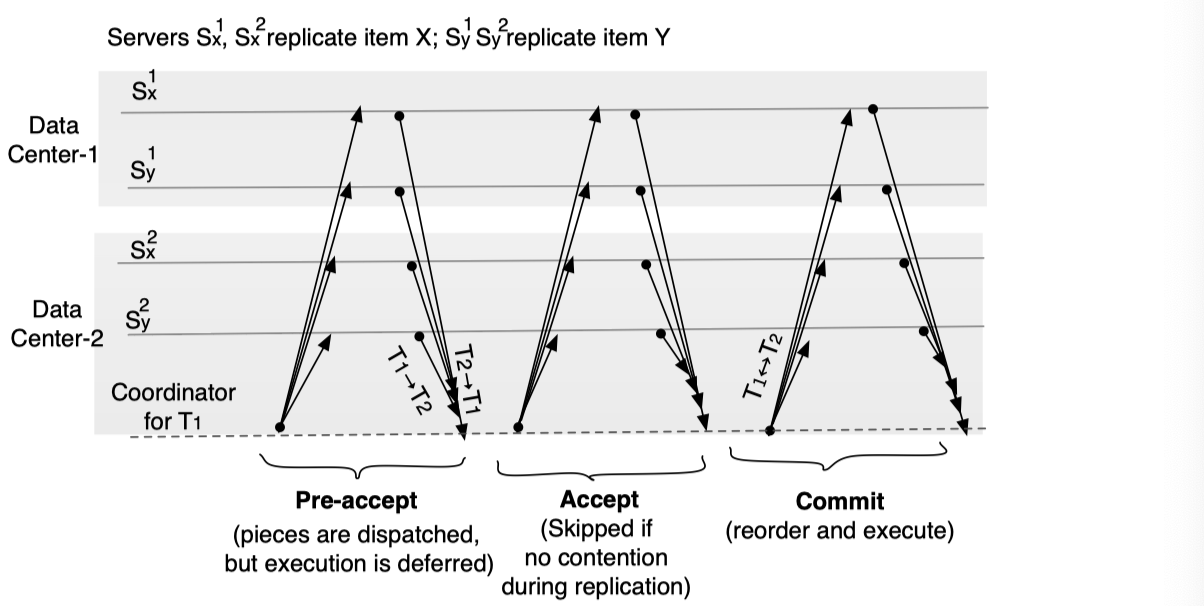
\includegraphics[width=0.8\textwidth]{Janus.png}
  \caption{Janus的三阶段协议}
  \label{fig:badge}
\end{figure}

(1)Pre-Accept 阶段,事务的组织者向所有参与者发起询问请求,各个参与者返回在本地生成且包含该事务的依赖图。组织者根据所有参与者的返回结果,判断协议的下一阶段内容。若所有参与者返回的依赖图相一致(将所以依赖图进行合并并检测合并后的依赖图中是否存在闭环),则协议可以直接进行commit阶段,否则需要和所有参与者商定一个最终结果,进入accept阶段。

\begin{figure}[htb]
  \centering
  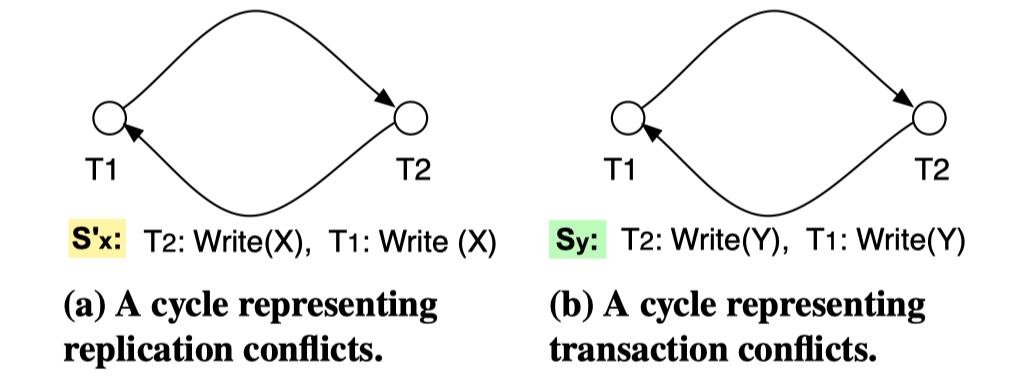
\includegraphics[width=0.8\textwidth]{Graph.png}
  \caption{整合后存在冲突的依赖图}
  \label{fig:badge}
\end{figure}

(2)Accept阶段,组织者选择一种合并的依赖关系并向所有参与者发起投票请求(ballot),所有参与者根据自身的情况选择accept/reject。若所有参与者都选择accept,则进入commit阶段。否则,组织者重新选取一种依赖关系,再进行投票。

(3)Commit阶段,组织者向所有参与者发起提交请求,所有参与者根据Accept阶段中接受的依赖关系执行事务。

需要注意的是第三阶段的commit不会给事务带了额外的WAN RTT,因为commit阶段事务的组织者只需要得到本地的commit指令得到回复就可以回复用户事务已经完成了,不同于二阶段提交(2PL)中的commit阶段,因为Janus在第二阶段或者第一阶段已经保证大多数的副本已经得到了一致的依赖关系。因此,即使此时事务的参与者宕机,在重启后,仍然能够根据已有的依赖图,执行事务。

Janus协议在没有冲突或者有冲突的事务在Pre-Accept的大多数中持有相同的依赖,则Janus只需要1个RTT来完成并发控制和共识协议的等效版本。否则,Janus需要执行额外的Accept阶段,来保证强一致性。

由于Janus只是实现了事务之间的依赖关系的序列化,那么如何保证事务的原子性呢?Janus对事务的模型进行了约束,Janus适用于能够将事务分解成多个存储过程,每个存储过程可以在各自的shard内独立完成,且彼此之间没有依赖关系,同时不存在程序逻辑或应用层引起的放弃提交操作。由此,Janus可以保证所有shard彼此独立的执行属于自己部分的事务内容,且不会违反原子性约束。并且,由于Janus适用事务组织者对每组冲突的事务都给出了最终依赖关系,且模型本身要求事务不会因为程序逻辑或应用层放弃提交,因此Janus的提交率总是100\%。

对于收到了完整的依赖关系却没有完整的实际事务参与者,何时才能执行事务呢?比如事务1被分发到参与者0,1上,事务2被分发到参与者1,2上,且根据参与者1的依赖图,组织者选择执行顺序为事务1、事务2,则参与者2会得到该依赖关系,但却没有实际的事务1的内容。此时Janus的做法是让参与者1就近询问其他参与者事务1的完成情况,若事务1完成,则可以执行。正是由于这个限制,Janus采用的全副本的模型,即所有数据中心都拥有所有shard 的完整副本,这样做的好处是,询问不会带来额外的WAN RTT。

另外,Janus 也可以对协议内容进行适当拓展,以支持事务的存储过程之间存在相互依赖(读写依赖)的模型,一个简单的做法是,在事务执行前检测这种依赖,并将写的存储过程先不执行,通过shard中间的交互,来获取读的数据,但这同样可能会引起额外的RTT。


\section{基于多版本的设计(Ocean Vista)}

Ocean Vista是时间戳的设计模型,利用数据存储多版本的方式实现并发控制,通过可见性约束(通过水印实现(watermark)),使得每个事务都只能看见且能看在在自己之前提交的所有事务,同时OV用异步的gossip实现跨数据中心的协作。Gossip的引入,缓解了每个事务执行时跨数据中心协作的必要。

首先,介绍gossip。Gossip是一种去中心化、容错并保证最终一致性的协议。它的基本思想是通过不断的和集群中的节点gossip交换信息,经过 O(log(n))个回合, gossip协议即可将信息传递到所有的节点。类似于,一个信息流在网络拓扑中,按相邻节点依次传递。需要注意的是,Gossip只保证了最终一致性,而OV利用它作为数据中心之间水印信息交换的协议,因此每个数据中心所持有的水印信息可能是不同的、陈旧的。

Ocean Vista 采用的架构如下图所示:

\begin{figure}[htb]
  \centering
  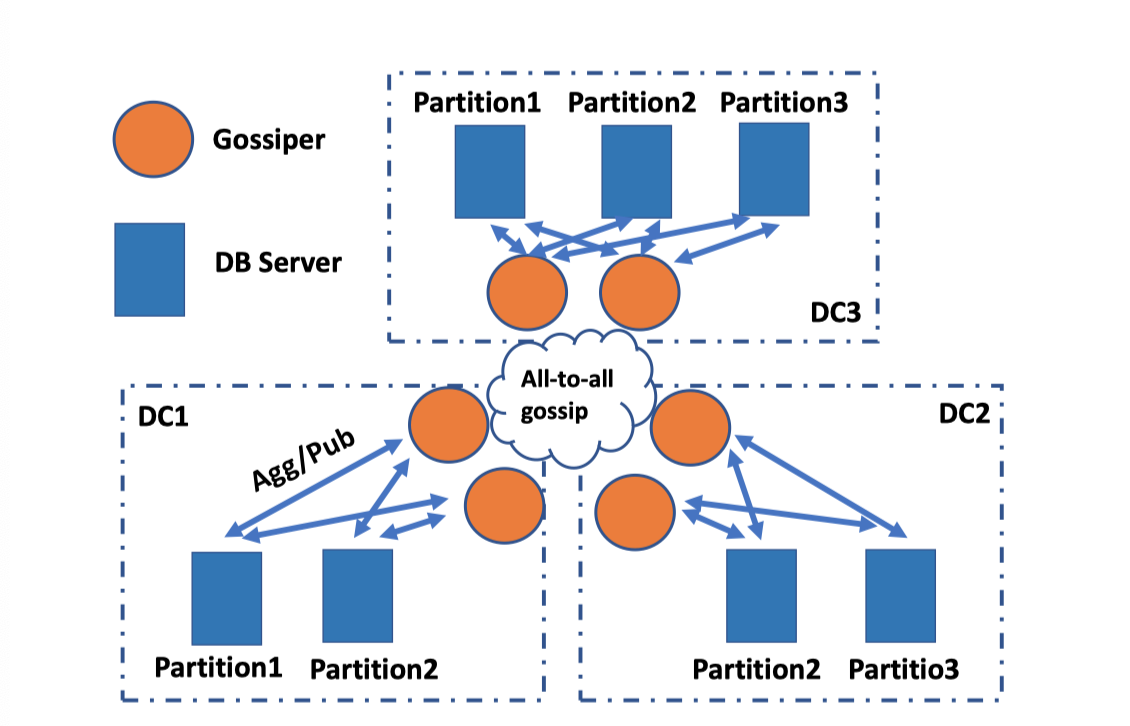
\includegraphics[width=0.8\textwidth]{OV-1.png}
  \caption{Ocean Vista整体架构}
  \label{fig:badge}
\end{figure}

每个数据中心的Gossiper 负责跨数据中心的通讯,事实上,每个数据中心只需要配备1个Gossiper,多个Gossiper的作用是为了实现容错和冗余。每个数据服务器提供了事务组织者、多版本数据维护、事务执行的功能。

Ocean Vista 定义了多个水印(水印是一个具体的版本号):

\begin{itemize}
\item Vwatermark:所有低于该版本号的事务应该都已经完成的预写阶段(S-phase)。
\item Rwatermark:所有低于该版本号的事务应该都已经在副本上完成备份。
\item svw:每个服务器(事务的组织者)维护的尚未可见的事务版本的最小值,也就是说该组织者发出的比该值小的事务都已经完成预写阶段(S-phase)。
\end{itemize}

具体来说,Ocean Vista 执行一个事务的流程如下图所示:

\begin{figure}[htb]
  \centering
  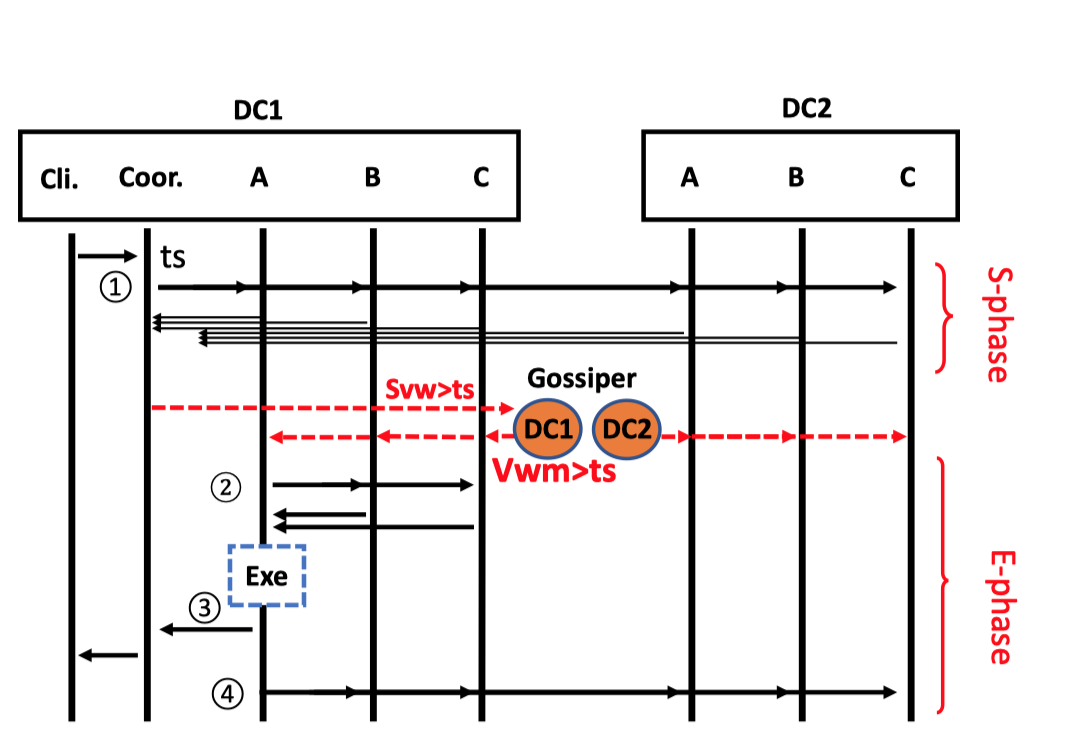
\includegraphics[width=0.8\textwidth]{OV_2.png}
  \caption{Ocean Vista事务处理流程}
  \label{fig:badge}
\end{figure}

首先,用户向一个数据中心的服务器发送事务请求,该服务器就作为该事务的组织者,该组者者使用全局唯一的序列号(基于同步时钟的单调递增序列),来给事务指派一个版本号。组织者在S-phase,将事务在数据库中占有一个全局唯一的版本号的占位符,该占位符具有该事务执行所需要的全部信息,但此时该信息对于其他事务是不可见的。直至,Gossop更新Vwatermark。需要注意的是这里,事务只是占用了一个占位符,但并没有真正执行,也没有读取执行所需要的数据。该占位符最终会被E-Phase阶段以后的具体的值所替代。当该事务在所有参与者上都完成了占位操作,组织者就可以将其加入到就绪列表。

Gossiper会持续的交换Vwatermark,所有具有比Vwatermark小的版本号的事务就已经准备好执行了。因为这表明此时这些事务已经在所有参与者上完成占位操作,也意味着可以按照版本顺序依次执行事务,而不会丢失之前的事务(因为之前的事务都已占位)。事务的读取的值可以从比该该事务版本号的前一个版本中直接读取。如果该事务的版本号比Rwatermark小,事务可以从最近的副本中读取数据,否则就需要从已经完成之前版本的副本上读取(需要额外的信息交互)。事务执行完成后,向组织者返回该事务的执行结果。并异步地将事务的执行结果在副本上备份,这一步的目的是使的副本能够尽快的得到最终结果,而不需要等待执行。

可以注意到的是,Ocean Vista 需要略大于1个RTT的时间来完成协议内容,因为可能需要等待gossip 的更新。除此之外,OV依赖于同步的时间戳来给定事务的执行顺序,并完成事务处理。相比于传统的时间戳方案,它使用gossip和多版本的存储系统实现了版本控制,取缔了二阶段提交协议(2PC)的使用。

在分布式系统中,维护同步的时钟往往是困难的,OV也采用了一系列的办法来修正时钟的偏移,由于这块内容不是本论文的重点,就不再赘述。


\section{基于局部性原理的设计(Slog)}

Slog基于分布式事务的局部性原理展开设计\cite{MasterPartition1},同时实现了强一致性、低时延的写任务和高吞吐量的目标。其采用的模型和大多数系统一致,即确定性的执行模型(determined model)。它继承了主-从副本的思想,即在同一个shard的所有副本中存在一个副本作为主副本。\cite{MasterPartition2}主副本负责实现事务的序列化,并负责与用户进行交互,其余副本只从主副本上同步数据,在主副本出现问题时,其余副本才开始负责处理用户请求。\cite{MasterPartition3}由于采用了确定性的执行模型,主副本只需要将所有序列化的事务同步给副本即可,而不需要同步所有的数据。根据确定性执行顺序,副本能够得到相同的一致结果。

Slog将事务分成两类:

\begin{itemize}
\item 单地区的事务
\item 多地区事务
\end{itemize}

Slog的一个前提条件是在执行某个事务前,知道该事务所要访问的所有数据(这个可以通过应用层协议简单实现)。用户向距离最近的数据中心提交事务请求,数据中心根据其所掌握的数据的归属信息(即被访问的数据的主副本的位置),来判断该事务属于单一地区事务或多地区事务。

对于单一地区事务,由于该事务所访问的所有数据的主副本位于同一个数据中心内,事务可以在该数据中心内完成执行并提交而不需要额外的跨数据中心的协作。同时,为了优化系统的吞吐量,slog采用了批处理的思想,将主副本和其他副本之间的同步分批进行,而不需要每执行一次就同步。但需要注意的是,主副本只有当该事务所属的批在所有其他所有副本上备份后,才能回复用户事务已经完成,这是为了避免主副本损坏而其余副本尚未收到同步信息的情况出现。

具体来说,slog每个副本维护一个本地的日志和一个全局日志\cite{Log},并根据收到的事务请求将自己负责的事务写入本地日志和全局日志,这一步也就完成了事务的序列化。并且接受来自其他数据库的同步信息并写入全局日志。如下图所示。除此之外,slog采用二阶段锁机制来保证事务的原子性。

\begin{figure}[htb]
  \centering
  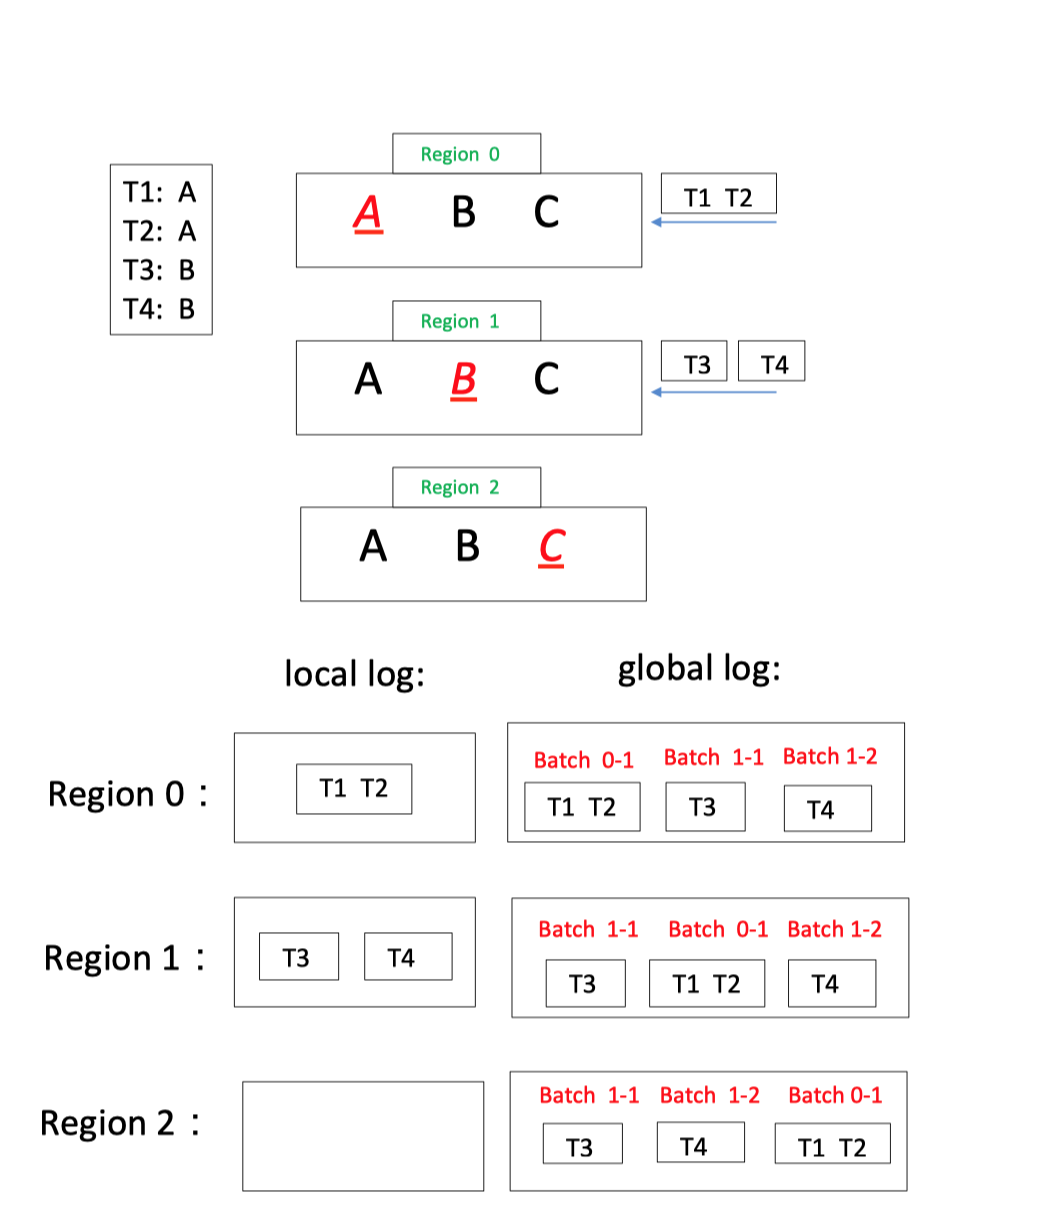
\includegraphics[width=0.6\textwidth]{slog_1.png}
  \caption{单地区事务处理}
  \label{fig:badge}
\end{figure}


对于多地区事务,slog通过一个中心节点的序列化方法或者利用paxos得到一个序列化的多地区事务的序列,
并根据这个序列中的顺序(可以是时间戳顺序或者任意的单调递增序列)将所有的多地区事务序列化。并根据事务所涉及的数据的归属信息,将事务拆分成多个小事务。这些细化后的事务被分配到各自的主副本上执行。这样以来也就确定了主副本上的单地区事务和多地区事务之间的顺序关系,从而形成了所用事务(包括:单地区事务和多地区事务)的全局序。

具体来说,事务的组织者发送事务到所有的主副本的数据中心,并写入本地日志,并根据取得锁的顺序依次执行,对于多地区任务执行完自的部分后还不能立刻提交,需要等到其收到所有该事务的细分事务的同步信息后才能提交该多地区事务。如下图所示:

\begin{figure}[htb]
  \centering
  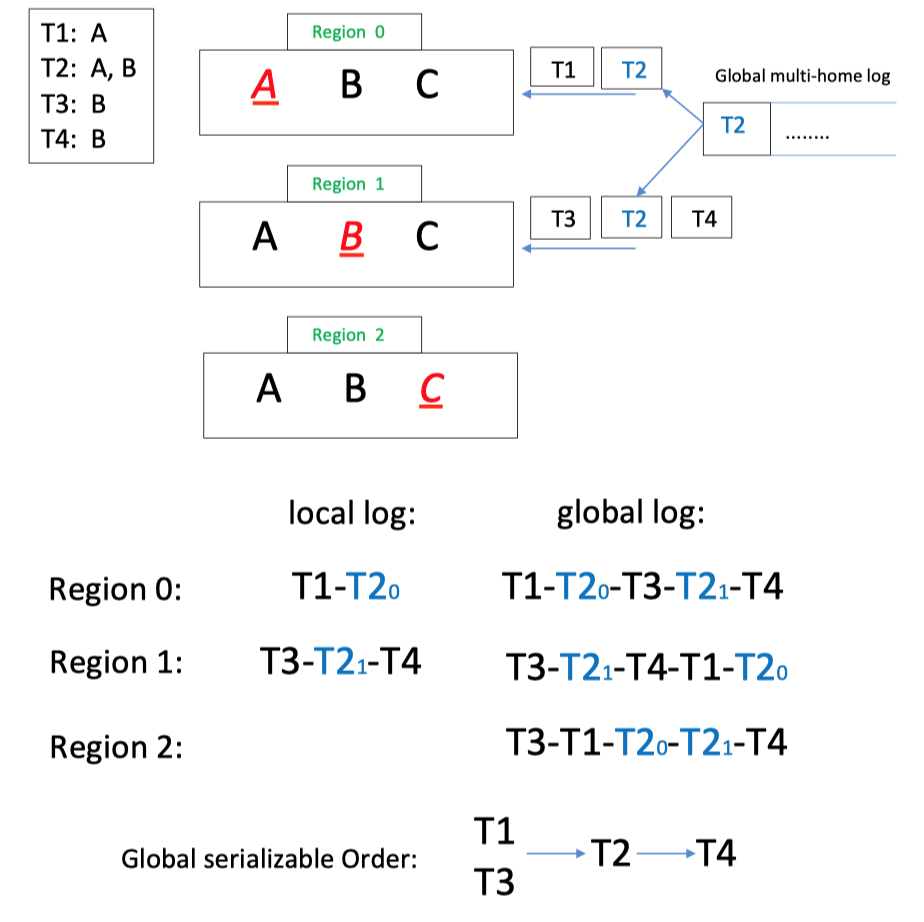
\includegraphics[width=0.6\textwidth]{slog_2.png}
  \caption{多地区事务处理}
  \label{fig:badge}
\end{figure}

虽然不同的地区执行事务的顺序不同,但他们所冲突的部分都被严格序列化。

显然,多地区事务的开销比单地区要大得多。因此,为了更好的维护数据的局部性,slog提供了主副本(即数据的归属信息)变更的方法,对于经常同时被访问的数据,slog更倾向于把数据的归属地区设置成一样的。这样,单地区事务的比例,在所有事务中得以增加。

Slog面临的一个问题是数据归属地的变更会使得每个地区维护的数据归属地的信息变的陈旧,slog的做法是如果事务根据陈旧的归属地信息到了一个不是数据的主副本的地区,这个事务放弃,并要求用户重新提交申请。同时,每个地区按照一定频率更新自己的归属信息表格。

Slog面临的另一个问题是多地区事务可能会阻塞单地区事务,因为多地区事务要在收齐该事务的所有细分事务后才能提交,这一过程会持续地占有锁,导致本地事务被阻塞。这可能会对系统性能带来不小的影响。

Slog利用全局日志和单一主副本的方法,保持的副本之间的一致性,因此不需要二阶段提交(2PL)这样的事务协议,但同时多地区事务的序列化要求了单一站点或者额外的共识协议,前者容易成为瓶颈,后者引入了额外的通讯开销。




\section{小结}

针对以上系统设计工作的分析,将各自对于活跃性(liveness)、在低冲突率和高冲突率的条件下的时延、可拓展性总结如下:

\begin{table}[htb]
  \centering\small
  \caption{各个系统之间的比较}
  \label{tab:exampletable}
  \begin{tabular}{ccccl}
    \toprule
    系统   & 活跃性(跨WAN的阻塞) & 低冲突率的时延 & 高冲突率的时延 & 可拓展性 \\
    \midrule
    TAPIR & 好 & 1RTT & Abort 并 retry & \\
    Janus & 中等*1 & 1 RTT &2RTT &坏*2  \\
    OceanVista & 坏 & 1RTT + $\Delta$&  1RTT+$\Delta$ &     \\
    Slog & 坏 & 1/2RTT + $\Delta$  &  1/2RTT + $\Delta$  &  \\
    \bottomrule
  \end{tabular}
\end{table}

*1 Janus在快速通道(Pre-Accept、Commit)时,Pre-Accept需要所有参与者的回复不冲突的结果,而不是大多数的参与者。

*2 当数据中心不具有所有shard 的完整备份时,Janus需要额外的WAN RTT。


结合现有系统的不足之处,对于之后的系统设计,我们提出了以下设计目标或设计原则:

\begin{itemize}
\item 单地区事务,即能够被单一数据中心处理的事务,应该尽可能减少跨区域的协作。从而减少WAN RTT的引入。
\item 单地区事务不应该被跨地区的事务所阻塞而饥饿。
\item 可拓展性要求,系统设计应是的随着shard 数目的增加,系统吞吐量近似与其表现为正相关。
\item 如果一个事务需要多个shard参与,那所有的协作都应该只发生在这些参与者之内。也就是说要尽可能减少不必要的参与者。
\end{itemize}








